\documentclass[11pt,a4paper]{article}

% ---------- Język i kodowanie ----------
\usepackage{iftex}
\ifPDFTeX                      % pdfLaTeX (m.in. domyslny silnik Overleafa)
  \usepackage[T1]{fontenc}
  \usepackage[utf8]{inputenc}
  \usepackage{lmodern}
  \newcommand{\tptimes}{\fontfamily{qtm}\selectfont}   % TeX Gyre Termes (Times)
\else                          % XeLaTeX / LuaLaTeX / Tectonic
  \usepackage{fontspec}
  \setmainfont{lmroman10-regular.otf}[
    BoldFont=lmroman10-bold.otf, ItalicFont=lmroman10-italic.otf,
    BoldItalicFont=lmroman10-bolditalic.otf]
  \setmonofont{lmmono10-regular.otf}
  \newfontfamily\tptimes{texgyretermes-regular.otf}[
    BoldFont=texgyretermes-bold.otf, ItalicFont=texgyretermes-italic.otf,
    BoldItalicFont=texgyretermes-bolditalic.otf]
\fi
\usepackage[polish]{babel}

% ---------- Matematyka, grafika, tabele ----------
\usepackage{amsmath}
\usepackage{amssymb}
\usepackage{graphicx}
\usepackage{booktabs}
\usepackage{float}
\usepackage{placeins}
\makeatletter
\setlength{\@fptop}{0pt}
\setlength{\@fpsep}{14pt plus 1fil}
\setlength{\@fpbot}{0pt plus 1fil}
\makeatother
\usepackage{caption}
\captionsetup[table]{position=top}
\captionsetup[figure]{position=bottom}
\usepackage{multirow}
\usepackage{array}
\usepackage{colortbl}
\usepackage[margin=2.5cm]{geometry}
\usepackage{pgfplots}
\pgfplotsset{compat=1.18}

% Barwy serii (rozróżnialne także w druku cz.-b. dzięki kształtom znaczników)
\definecolor{seriaA}{HTML}{1F5FA9}   % niebieski  -- linia L1
\definecolor{seriaB}{HTML}{C62828}   % czerwony   -- linia N
\definecolor{limQP}{HTML}{333333}    % poziom dopuszczalny QP
\definecolor{limAV}{HTML}{E07B00}    % poziom dopuszczalny AV
\pgfplotsset{
  wykres/.style={
    width=15.2cm, height=8.4cm, grid=major,
    grid style={line width=0.2pt, draw=gray!18},
    major grid style={line width=0.35pt, draw=gray!30},
    xmin=0.15, xmax=30,
    xlabel={Częstotliwość $f$ [MHz]},
    xtick={0.15,0.2,0.3,0.5,1,2,3,5,10,20,30},
    xticklabels={{0,15},{0,2},{0,3},{0,5},1,2,3,5,10,20,30},
    ylabel={Poziom zaburzeń $U$ [dB\textmu V]},
    y tick label style={/pgf/number format/use comma},
    legend cell align=left,
    legend style={font=\small, fill=white, draw=gray!40, at={(0.5,0)}, anchor=north, yshift=-1.25cm,
                  /tikz/every even column/.append style={column sep=1.0em}},
    title style={font=\small, yshift=0.2em},
    tick label style={font=\small}, label style={font=\small}
  }
}
% poziomy dopuszczalne PN-EN 55032 kl. B (w 0,15-0,5 MHz liniowo względem log f)
\newcommand{\limity}{%
  \addplot[line width=1.2pt, limQP] coordinates {(0.15,66) (0.5,56) (5,56) (5,60) (30,60)};
  \addlegendentry{poziom dopuszczalny QP}
  \addplot[line width=1.2pt, limAV, dashed] coordinates {(0.15,56) (0.5,46) (5,46) (5,50) (30,50)};
  \addlegendentry{poziom dopuszczalny AV}}
\usepackage[hidelinks,unicode]{hyperref}
\emergencystretch=1em
% Wstawianie wierszy tabel z plików: prymityw TeX-a działa w tabular przed \bottomrule
\makeatletter\newcommand{\tabinput}[1]{\@@input #1.tex }\makeatother
\newcommand{\dBuV}{\text{dB\textmu V}}

% ---------- Strona tytułowa: odwzorowanie Szablon_strony_tytulowej_LKEMBEM.doc ----------
\newcolumntype{Y}[1]{>{\centering\arraybackslash}m{#1}}
\newcolumntype{Z}[1]{>{\raggedright\arraybackslash}m{#1}}
\newcolumntype{W}[1]{>{\raggedright\arraybackslash}p{#1}}
\newlength{\tpw}\newlength{\tpt}
\newlength{\tpcA}\newlength{\tpcB}\newlength{\tpcC}
\newlength{\tpAB}\newlength{\tpBC}\newlength{\tpABC}
\newlength{\tpsig}
\newcommand{\tplengths}{%
  \setlength{\tabcolsep}{5pt}%
  \setlength{\arrayrulewidth}{0.5pt}%
  \setlength{\tpw}{\dimexpr\textwidth-4\arrayrulewidth-6\tabcolsep-1pt\relax}%
  \setlength{\tpcA}{0.4966\tpw}%
  \setlength{\tpcB}{0.2481\tpw}%
  \setlength{\tpcC}{0.2553\tpw}%
  \setlength{\tpAB}{\dimexpr\tpcA+\tpcB+2\tabcolsep+\arrayrulewidth\relax}%
  \setlength{\tpBC}{\dimexpr\tpcB+\tpcC+2\tabcolsep+\arrayrulewidth\relax}%
  \setlength{\tpABC}{\dimexpr\tpAB+\tpcC+2\tabcolsep+\arrayrulewidth\relax}%
  \setlength{\tpsig}{\dimexpr(\tpABC-2\arrayrulewidth)/3\relax}}
\newcommand{\tph}[1]{\setlength{\tpt}{#1}\rule[-0.5\tpt]{0pt}{\tpt}}

% ---------- Dane do strony tytułowej (trzech równorzędnych autorów, kolejność alfabetyczna) ----------
\newcommand{\tpTermin}{PN/N, 15.15 - 18.45}
\newcommand{\tpGrupa}{5}
\newcommand{\tpCwiczenie}{2}
\newcommand{\tpTemat}{Pomiary przewodzonych zaburzeń elektromagnetycznych za pomocą sieci sztucznej}
\newcommand{\tpDataWyk}{09.11.2026}
\newcommand{\tpDataOdd}{21.11.2026}
\newcommand{\tpWersja}{Oryginał}
\newcommand{\tpOsobaA}{Wiktor Gruszczyński, 283808}
\newcommand{\tpOsobaB}{Nikodem Konieczny, 283838}
\newcommand{\tpOsobaC}{Filip Rodziewicz, 283825}
\newcommand{\tpPodpisA}{Wiktor Gruszczyński}
\newcommand{\tpPodpisB}{Nikodem Konieczny}
\newcommand{\tpPodpisC}{Filip Rodziewicz}

\newcommand{\stronatytulowa}{%
\begin{titlepage}
\thispagestyle{empty}
\tptimes\fontsize{12}{14.4}\selectfont
\tplengths
\arrayrulecolor[HTML]{BFBFBF}
\noindent
\begin{tabular}{|Z{\tpcA}|Z{\tpcB}|Z{\tpcC}|}
\hline
\multicolumn{3}{|Y{\tpABC}|}{%
  \textbf{\textsc{Politechnika Wrocławska}}\newline
  \textbf{\textsc{Katedra Telekomunikacji i~Teleinformatyki}}} \\
\hline
\multicolumn{1}{|Y{\tpcA}|}{\vspace*{3pt}%
  \textbf{\textsc{Bezpieczeństwo elektromagnetyczne}}\vspace*{3pt}} &
\multicolumn{2}{Y{\tpBC}|}{\textsc{Termin zajęć: \tpTermin}} \\
\hline
\tph{20pt}\textsc{Nr grupy:} \textbf{\tpGrupa} &
\multicolumn{2}{Z{\tpBC}|}{\textsc{Nr ćwiczenia:} \textbf{\tpCwiczenie}} \\
\hline
\multicolumn{1}{|W{\tpcA}|}{%
  \textsc{Skład grupy:}\newline
  \textsc{\tpOsobaA}\newline
  \textsc{\tpOsobaB}\newline
  \textsc{\tpOsobaC}\vspace*{6pt}} &
\multicolumn{2}{W{\tpBC}|}{\multirow[t]{3}{\tpBC}{%
  \textsc{Temat ćwiczenia:}\newline
  \textbf{\textsc{\tpTemat}}}} \\
\cline{1-1}
\multicolumn{1}{|Z{\tpcA}|}{\tph{22pt}%
  \textsc{Data wykonania ćw.:} \textbf{\tpDataWyk}} &
\multicolumn{2}{Z{\tpBC}|}{} \\
\cline{1-1}
\multicolumn{1}{|Z{\tpcA}|}{\vspace*{3pt}%
  \textsc{Wersja sprawozdania:}\newline
  \hfill\textbf{\textsc{\tpWersja}}\vspace*{3pt}} &
\multicolumn{2}{Z{\tpBC}|}{} \\
\hline
\multicolumn{2}{|Z{\tpAB}|}{\tph{26pt}\textsc{Data oddania sprawozdania:} \textbf{\tpDataOdd}} &
  \textsc{Ocena:} \\
\hline
\multicolumn{3}{|Y{\tpABC}|}{\tph{26pt}%
  \textbf{Zapoznałem się z~niniejszym sprawozdaniem i~uważam je za wykonane poprawnie.}} \\
\hline
\multicolumn{3}{|Y{\tpABC}|}{\setlength{\tabcolsep}{0pt}%
  \begin{tabular}{@{}Y{\tpsig}|Y{\tpsig}|Y{\tpsig}@{}}
    \tph{28pt}\fontsize{10}{12}\selectfont\tpPodpisA &
    \fontsize{10}{12}\selectfont\tpPodpisB &
    \fontsize{10}{12}\selectfont\tpPodpisC
  \end{tabular}} \\
\hline
\end{tabular}
\arrayrulecolor{black}
\end{titlepage}}

% Wspólny nagłówek tabel z wynikami pomiaru końcowego
\newcommand{\naglKoncowy}{%
  $f$ & Detektor & $U$ & $L$ & $\Delta = U - L$ & Ocena \\
  $[\mathrm{kHz}]$ & & [\dBuV] & [\dBuV] & [dB] & \\}
% Zrzut ekranu odbiornika z podpisem a)/b)
\newcommand{\ekranw}[3]{\begin{minipage}[t]{#1\textwidth}\centering
    \includegraphics[width=\linewidth]{rys/#2.png}\\{\small #3}\end{minipage}}
\newcommand{\ekran}[2]{\begin{minipage}[t]{0.485\textwidth}\centering
    \includegraphics[width=\linewidth]{rys/#1.png}\\{\small #2}\end{minipage}}

\addto\captionspolish{\renewcommand{\refname}{Bibliografia}}
\begin{document}
\stronatytulowa

\section{Cel ćwiczenia}

Celem ćwiczenia było zapoznanie się z~techniką pomiaru przewodzonych zaburzeń
elektromagnetycznych w~paśmie $150\ \mathrm{kHz}$--$30\ \mathrm{MHz}$ z~wykorzystaniem sieci
sztucznej i~odbiornika pomiarowego oraz ocena zgodności badanych urządzeń z~normą PN-EN~55032.

Badaniom poddano zasilacz sieciowy USB-A pracujący bez obciążenia, z~aparatem oraz z~lampką
LED zasilaną z~gniazda USB-A. Dodatkowo zmierzono ładowarkę Apple USB-C bez obciążenia
oraz podczas ładowania telefonu iPhone.

\section{Stanowisko pomiarowe}

\subsection{Metoda pomiarowa}

Pomiary wykonano metodą opisaną w~normie PN-EN~55016-2-1. Badane urządzenie (EUT) zasilane
jest przez sieć sztuczną (AMN), która zapewnia określoną impedancję sieci
($50\ \Omega$ równolegle z~$50\ \mu\mathrm{H} + 5\ \Omega$ względem ziemi), tłumi zaburzenia
pochodzące z~sieci zasilającej i~wyprowadza napięcie zaburzeń do odbiornika.

Mierzone jest napięcie między przewodem L1 lub N a~ziemią, przy czym linię wybiera się
przełącznikiem sieci sztucznej. Napięcie to zawiera składową różnicową (DM) i~wspólną (CM):
\begin{equation}
  U_{DM} = \tfrac{1}{2}\,(U_{L1} - U_{N}), \qquad U_{CM} = \tfrac{1}{2}\,(U_{L1} + U_{N}).
  \label{eq:dmcm}
\end{equation}

Pomiar jest dwuetapowy. W~pomiarze wstępnym pasmo przemiatane jest detektorami wartości
szczytowej (PK) i~średniej (AV). Na częstotliwościach, na których poziom zaburzeń zbliża się do
poziomu dopuszczalnego na mniej niż $6\ \mathrm{dB}$, odbiornik wykonuje pomiar końcowy
detektorami quasi-szczytowym (QP) i~AV z~czasem pomiaru $2\ \mathrm{s}$.

Ponieważ $U_{PK} \ge U_{QP} \ge U_{AV}$, wyniki wstępne niższe od poziomów dopuszczalnych
o~ponad $6\ \mathrm{dB}$ pozwalają stwierdzić zgodność bez pomiaru końcowego.

\subsection{Konfiguracja stanowiska pomiarowego}

\subsubsection{Spis aparatury pomiarowej}

\begin{table}[H]
  \centering
  \small
  \caption{Spis aparatury i~wyposażenia stanowiska pomiarowego.}
  \label{tab:aparatura}
  \renewcommand{\arraystretch}{1.25}
  \begin{tabular}{|c|>{\raggedright\arraybackslash}p{4.6cm}|>{\raggedright\arraybackslash}p{8.2cm}|}
    \hline
    \textbf{Lp.} & \textbf{Nazwa przyrządu / elementu} & \multicolumn{1}{c|}{\textbf{Model lub typ, uwagi}} \\
    \hline
    1 & Odbiornik pomiarowy & Rohde \& Schwarz ESL3, EMI Test Receiver, $9\ \mathrm{kHz}$--$3\ \mathrm{GHz}$,
        oprogramowanie 1.83 SP1 \\
    \hline
    2 & Sieć sztuczna (AMN) & dwuprzewodowa sieć typu V $50\ \Omega/50\ \mu\mathrm{H}$, przełącznik
        linii L1/N, dławik przewodu ochronnego (\emph{Earth Line Choke}), zacisk uziemienia
        w.cz. \\
    \hline
    3 & Ogranicznik impulsów (\emph{pulse limiter}) & zabezpieczenie wejścia odbiornika,
        tłumienie kompensowane przetwornikiem \texttt{PULS\_LIM} \\
    \hline
    4 & Przewody & współosiowy $50\ \Omega$ (AMN--odbiornik), przewód zasilający EUT zakończony gniazdem \\
    \hline
    5 & Stół pomiarowy & stół drewniany, EUT w~odległości ok.~$0{,}8\ \mathrm{m}$ od sieci sztucznej \\
    \hline
    6 & Badane urządzenia & zasilacz sieciowy USB-A (,,kostka'') bez oznaczenia modelu, ładowarka Apple USB-C;
        obciążenia: aparat, lampka LED USB-A, telefon iPhone \\
    \hline
  \end{tabular}
\end{table}

\subsubsection{Opis konfiguracji}

Stanowisko zestawiono według schematu zalecanego w~normie i~w~instrukcji do ćwiczenia
(rys.~\ref{fig:stanowisko}a). Badane urządzenie umieszczono na stole w~odległości
ok.~$0{,}8\ \mathrm{m}$ od sieci sztucznej, co mieści się w~zalecanym zakresie
$0{,}8$--$1\ \mathrm{m}$.

Zasilacze wpinano do gniazda na końcu przewodu wyprowadzonego z~sieci sztucznej
(rys.~\ref{fig:stanowisko}b). Przewód ułożono poziomo na stole; jego długość była zbliżona do
odległości EUT od sieci sztucznej, dlatego nie było potrzeby układania nadmiaru w~meandry.
Wyjście sieci sztucznej połączono z~odbiornikiem przez ogranicznik impulsów i~przewód
współosiowy, poprowadzony z~dala od przewodów EUT.

Zachowano zalecane odległości EUT od płaszczyzny odniesienia ($0{,}4\ \mathrm{m}$) oraz od
innych uziemionych powierzchni (co najmniej $0{,}8\ \mathrm{m}$). Ma to znaczenie, ponieważ
badane zasilacze nie mają przewodu ochronnego, a~składowa wspólna zaburzeń zamyka się przez
pojemności pasożytnicze względem ziemi.

\begin{figure}[H]
  \centering
  \begin{minipage}[b]{0.49\textwidth}\centering
    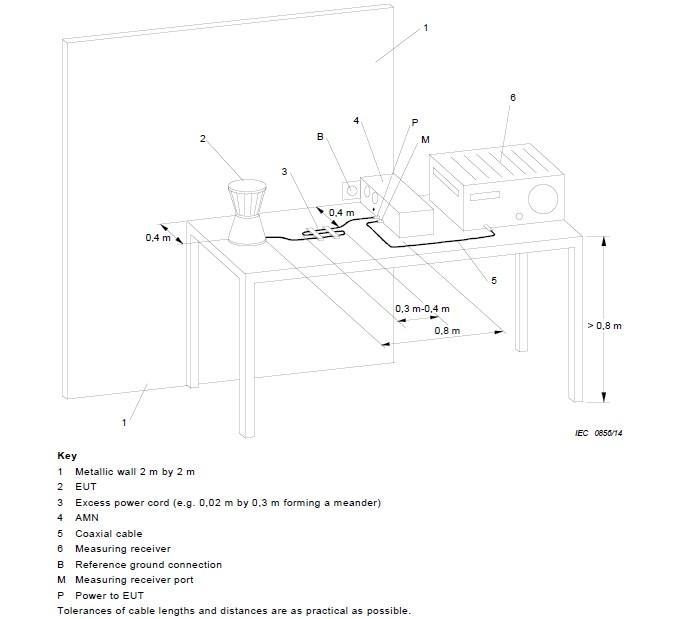
\includegraphics[width=\linewidth]{rys/schemat_stanowiska.png}\\
    {\small a) schemat wg PN-EN~55016-2-1 (instrukcja do ćwiczenia, rys.~2-2)}
  \end{minipage}\hfill
  \begin{minipage}[b]{0.49\textwidth}\centering
    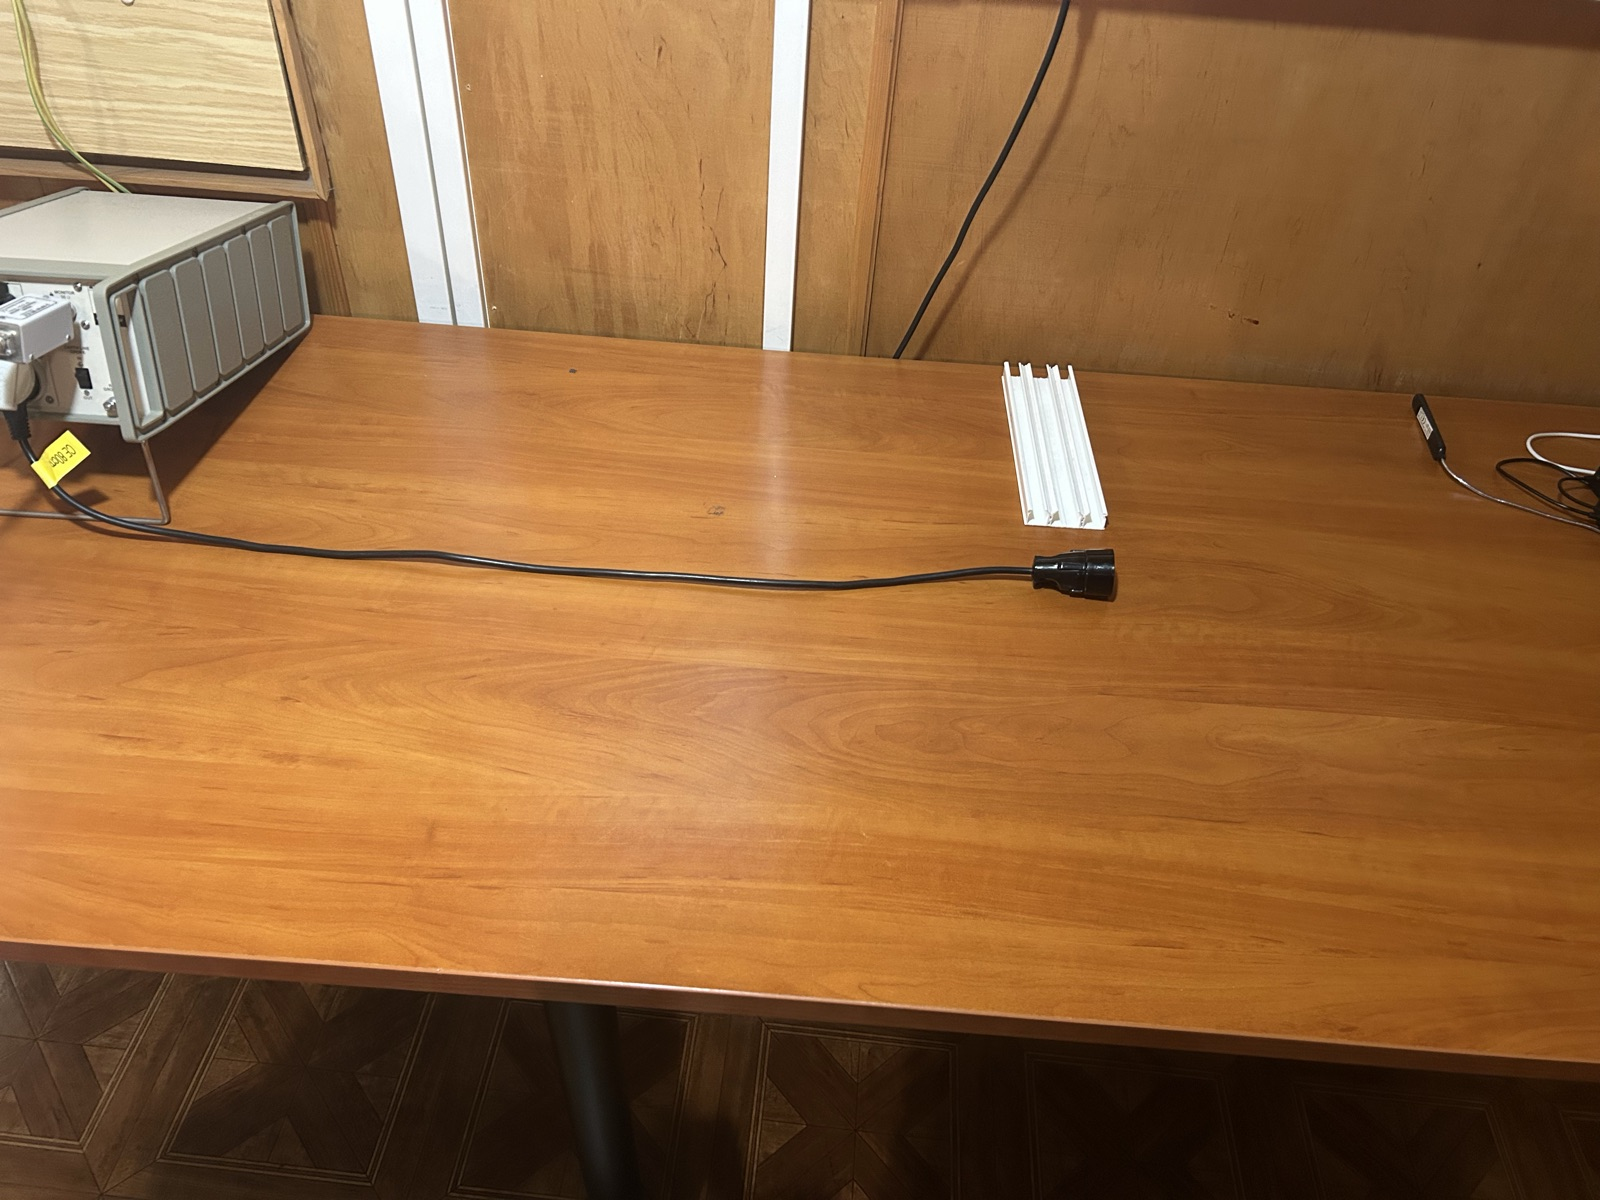
\includegraphics[width=\linewidth]{rys/stanowisko_bez_eut.jpg}\\
    {\small b) sieć sztuczna przy krawędzi stołu i~przewód zasilający EUT, zdjęcie własne}
  \end{minipage}
  \caption{Stanowisko do pomiaru zaburzeń przewodzonych w~sali~347 bud.~C-4.}
  \label{fig:stanowisko}
\end{figure}

\section{Realizacja ćwiczenia}

\subsection{Nastawy odbiornika pomiarowego}

Odbiornik skonfigurowano zgodnie z~uproszczoną instrukcją obsługi. Śladowi~1 przypisano
detektor PK w~pomiarze wstępnym i~QP w~pomiarze końcowym, a~śladowi~2 detektor AV w~obu
etapach. Pozostałe nastawy odbiornika ustawiono zgodnie z~tabelą~\ref{tab:nastawy}.

\begin{table}[H]
  \centering
  \small
  \caption{Nastawy odbiornika pomiarowego R\&S ESL3.}
  \label{tab:nastawy}
  \renewcommand{\arraystretch}{1.15}
  \begin{tabular}{|l|l|}
    \hline
    \textbf{Parametr} & \textbf{Wartość} \\
    \hline
    Tryb pracy                         & \emph{Receiver}, skanowanie wg tabeli (\emph{Scan Table}) \\
    \hline
    Zakres częstotliwości              & $150\ \mathrm{kHz}$--$30\ \mathrm{MHz}$, oś logarytmiczna \\
    \hline
    Krok / szerokość pasma RBW         & $4\ \mathrm{kHz}$ / $9\ \mathrm{kHz}$ \\
    \hline
    Czas pomiaru w~kroku (pomiar wstępny) & $30\ \mathrm{ms}$ \\
    \hline
    Tłumik RF / przedwzmacniacz / \emph{Auto Ranging} & $10\ \mathrm{dB}$ / wyłączony / wyłączone \\
    \hline
    Detektory: pomiar wstępny          & ślad 1: PK (\emph{Max Peak}), ślad 2: AV \\
    \hline
    Detektory: pomiar końcowy          & ślad 1: QP, ślad 2: AV \\
    \hline
    Czas pomiaru końcowego             & $2\ \mathrm{s}$ \\
    \hline
    Margines wyboru częstotliwości     & $6\ \mathrm{dB}$ \\
    \hline
    Przetwornik (kompensacja toru)     & \texttt{PULS\_LIM} (ogranicznik impulsów) \\
    \hline
    Poziomy dopuszczalne               & EN55032 QP, EN55032 AV (klasa B) \\
    \hline
  \end{tabular}
\end{table}

Czas pomiaru w~kroku ustawiono na $30\ \mathrm{ms}$ zamiast podanych w~instrukcji
$50\ \mathrm{ms}$, zgodnie z~poleceniem prowadzącego, co skróciło czas pomiaru wstępnego. Zaburzenia
zasilaczy impulsowych powtarzają się z~okresem przełączania (ok.~$17\ \mu\mathrm{s}$) i~z~okresem
sieci ($20\ \mathrm{ms}$), dlatego czas $30\ \mathrm{ms}$ obejmuje pełny okres modulacji i~nie ma
istotnego wpływu na wynik.

W~tabeli przetworników aktywny był tylko ogranicznik impulsów; współczynnika podziału sieci
sztucznej i~tłumienia przewodu nie uwzględniono. W~pomiarach~5 i~6 detektor końcowy śladu~1
był ustawiony na PK, co nie wpłynęło na wynik, gdyż odbiornik nie wytypował wtedy żadnej
częstotliwości do pomiaru końcowego.

\FloatBarrier
\subsection{Przebieg pomiarów}

Zgodnie z~instrukcją najpierw zmierzono tło bez badanego urządzenia, a~następnie zasilacze
bez obciążenia i~z~obciążeniem (tab.~\ref{tab:pomiary}). Pomiary~1--8 wykonano na linii L1,
a~pomiary~9 i~10 na linii N (rys.~\ref{fig:przelacznik}).

Ładowarkę Apple badano w~pomiarach~3 i~4, bez obciążenia i~podczas ładowania telefonu.
W~pozostałych pomiarach z~EUT użyto tego samego zasilacza USB-A, zmieniając jedynie przewód USB
i~obciążenie. Zrzuty
ekranu zapisano dla wszystkich pomiarów, a~listy wyników końcowych dla pomiarów~5--10.

\begin{table}[H]
  \centering
  \small
  \caption{Wykaz wykonanych pomiarów w~kolejności wykonania.}
  \label{tab:pomiary}
  \renewcommand{\arraystretch}{1.2}
  \begin{tabular}{|c|>{\raggedright\arraybackslash}p{8cm}|c|}
    \hline
    \textbf{Nr} & \textbf{Badane urządzenie / obciążenie} & \textbf{Linia} \\
    \hline
    1  & brak EUT (pomiar szumów i~tła) & L1 \\ \hline
    2  & zasilacz USB-A bez przewodu i~obciążenia & L1 \\ \hline
    3  & ładowarka Apple USB-C z~przewodem, bez obciążenia & L1 \\ \hline
    4  & ładowarka Apple USB-C, ładowanie telefonu iPhone & L1 \\ \hline
    5  & zasilacz USB-A bez obciążenia, przed podłączeniem aparatu & L1 \\ \hline
    6  & zasilacz USB-A z~podłączonym aparatem & L1 \\ \hline
    7  & zasilacz USB-A bez przewodu i~obciążenia, przed podłączeniem lampki & L1 \\ \hline
    8  & zasilacz USB-A z~lampką LED USB-A & L1 \\ \hline
    9  & zasilacz USB-A z~lampką LED USB-A & N  \\ \hline
    10 & zasilacz USB-A bez przewodu i~obciążenia, po odłączeniu lampki & N  \\ \hline
  \end{tabular}
\end{table}

\subsection{Poziomy dopuszczalne i~kryterium oceny}

Poziom napięcia zaburzeń wyrażany jest w~decybelach względem $1\ \mu\mathrm{V}$:
\begin{equation}
  U\,[\dBuV] = 20\log_{10}\frac{U}{1\ \mu\mathrm{V}}.
  \label{eq:dbuv}
\end{equation}
Poziomy dopuszczalne zaburzeń przewodzonych na porcie zasilania według PN-EN~55032 podano
w~tabeli~\ref{tab:limity}. W~paśmie $0{,}15$--$0{,}5\ \mathrm{MHz}$ poziom dopuszczalny maleje
liniowo względem logarytmu częstotliwości:
\begin{equation}
  L_{QP}(f) = 66 - 10\,\frac{\log_{10}(f/0{,}15\ \mathrm{MHz})}{\log_{10}(0{,}5/0{,}15)}\ [\dBuV],
  \qquad L_{AV}(f) = L_{QP}(f) - 10\ \mathrm{dB}.
  \label{eq:limit}
\end{equation}
Odstęp wyniku od poziomu dopuszczalnego określa zależność
\begin{equation}
  \Delta = U - L\ [\mathrm{dB}].
  \label{eq:delta}
\end{equation}
Urządzenie uznaje się za zgodne z~wymaganiami, jeżeli dla wszystkich wyników pomiaru
końcowego, zarówno dla detektora QP, jak i~AV, spełniony jest warunek $\Delta \le 0$. Gdy pomiar końcowy nie był wykonywany, kryterium
zastosowano do wyników wstępnych (ślad PK względem $L_{QP}$, ślad AV względem $L_{AV}$).

\begin{table}[H]
  \centering
  \small
  \caption{Poziomy dopuszczalne zaburzeń przewodzonych wg PN-EN~55032.}
  \label{tab:limity}
  \renewcommand{\arraystretch}{1.15}
  \begin{tabular}{|c|c|c|}
    \hline
    \textbf{Zakres częstotliwości} & \textbf{Detektor QP [\dBuV]} & \textbf{Detektor AV [\dBuV]} \\
    \hline
    $0{,}15$--$0{,}5\ \mathrm{MHz}$ & $66$--$56$ & $56$--$46$ \\ \hline
    $0{,}5$--$5\ \mathrm{MHz}$      & $56$       & $46$ \\ \hline
    $5$--$30\ \mathrm{MHz}$         & $60$       & $50$ \\ \hline
  \end{tabular}
\end{table}

Niepewność pomiaru zaburzeń przewodzonych w~paśmie $150\ \mathrm{kHz}$--$30\ \mathrm{MHz}$
wynosi wg PN-EN~55016-4-2 $U_{cispr} = 3{,}4\ \mathrm{dB}$. Jeżeli niepewność laboratorium nie
przekracza tej wartości, o~zgodności rozstrzyga bezpośrednie porównanie wyniku z~poziomem
dopuszczalnym.

\section{Opracowanie wyników}
\label{sec:analiza}

\subsection{Pomiar szumów i~tła}
\label{sec:tlo}

Bez badanego urządzenia (rys.~\ref{fig:ekr-tlo}a) poziom tła do $3\ \mathrm{MHz}$ wynosił
ok.~$37$--$38\ \dBuV$ dla detektora PK i~ok.~$27\ \dBuV$ dla AV. Przy ok.~$3\ \mathrm{MHz}$ oba
ślady rosną skokowo o~ok.~$4\ \mathrm{dB}$, a~powyżej maleją do ok.~$31\ \dBuV$ (PK)
i~$20\ \dBuV$ (AV) przy $30\ \mathrm{MHz}$. Widoczne są też wąskie prążki przy ok.~$5{,}4$
i~$10\ \mathrm{MHz}$.

Skok i~prążki występują we wszystkich pomiarach, również bez EUT, pochodzą więc z~odbiornika lub
otoczenia. Tło leży co najmniej ok.~$13\ \mathrm{dB}$ poniżej poziomów dopuszczalnych, co umożliwia
ocenę zgodności. Przebieg dla samego zasilacza USB-A (pomiar~2) nie różni się od tła.

\begin{figure}[H]
  \centering
  \ekran{ekr_1_szum}{a) pomiar 1: bez EUT}\hfill
  \ekran{ekr_2_kostka}{b) pomiar 2: sam zasilacz USB-A}
  \caption{Pomiar wstępny, linia L1. Ślad żółty:
           detektor PK, niebieski: AV, linie czerwone: poziomy dopuszczalne EN55032 QP i~AV.}
  \label{fig:ekr-tlo}
\end{figure}

\subsection{Ładowarka Apple i~zasilacz z~aparatem}
\label{sec:aparat}

Ładowarka Apple bez obciążenia (pomiar~3, rys.~\ref{fig:ekr-kostka}a) daje przebieg
nieodróżnialny od tła. W~przeciwieństwie do tego, podczas ładowania telefonu
(rys.~\ref{fig:ekr-kostka}b) ładowarka wytwarza zauważalne zaburzenia w~paśmie $0{,}15$--$0{,}5\ \mathrm{MHz}$. Najwyższy prążek PK,
ok.~$57\ \dBuV$ przy ok.~$200\ \mathrm{kHz}$, leży ok.~$6\ \mathrm{dB}$ poniżej
$L_{QP} = 63{,}6\ \dBuV$, a~prążek AV (ok.~$41\ \dBuV$) ok.~$12\ \mathrm{dB}$ poniżej
$L_{AV} = 53{,}6\ \dBuV$. Margines PK leży na granicy progu $6\ \mathrm{dB}$, jednak odbiornik nie
wytypował częstotliwości do pomiaru końcowego, a~wszystkie testy zakończyły się wynikiem PASS. Ładowarka Apple z~obciążeniem spełnia wymagania normy.

\begin{figure}[H]
  \centering
  \ekran{ekr_3_kostka_kabel}{a) pomiar 3: bez obciążenia}\hfill
  \ekran{ekr_4_apple}{b) pomiar 4: ładowanie iPhone'a}
  \caption{Pomiar wstępny ładowarki Apple, linia L1.}
  \label{fig:ekr-kostka}
\end{figure}

W~pomiarach~5 (sam zasilacz) i~6 (zasilacz z~aparatem) przebiegi pokrywają się z~tłem w~niemal
całym paśmie (rys.~\ref{fig:ekr-aparat}). W~pomiarze~5 pojawił się jedynie prążek PK
ok.~$42\ \dBuV$ przy ok.~$12\ \mathrm{MHz}$, obecny w~różnym stopniu w~pomiarach~2--6. Po podłączeniu aparatu wystąpiły wzniesienia do
ok.~$41\ \dBuV$ w~paśmie $18$--$28\ \mathrm{MHz}$. Oba przebiegi leżą co najmniej
ok.~$17\ \mathrm{dB}$ poniżej poziomu QP.

Żaden wynik wstępny nie zbliżył się do poziomu dopuszczalnego na mniej niż $6\ \mathrm{dB}$,
dlatego odbiornik nie wykonał pomiaru końcowego, a~pliki \texttt{.DAT} zawierają pustą listę
wyników (\texttt{Values;0}). Zasilacz USB-A z~aparatem spełnia wymagania PN-EN~55032 dla
klasy~B.

\begin{figure}[H]
  \centering
  \ekran{ekr_5_aparat}{a) pomiar 5: sam zasilacz}\hfill
  \ekran{ekr_6_aparat_podpiety}{b) pomiar 6: zasilacz z~aparatem}\\[8pt]
  \begin{minipage}[t]{0.5\textwidth}\centering
    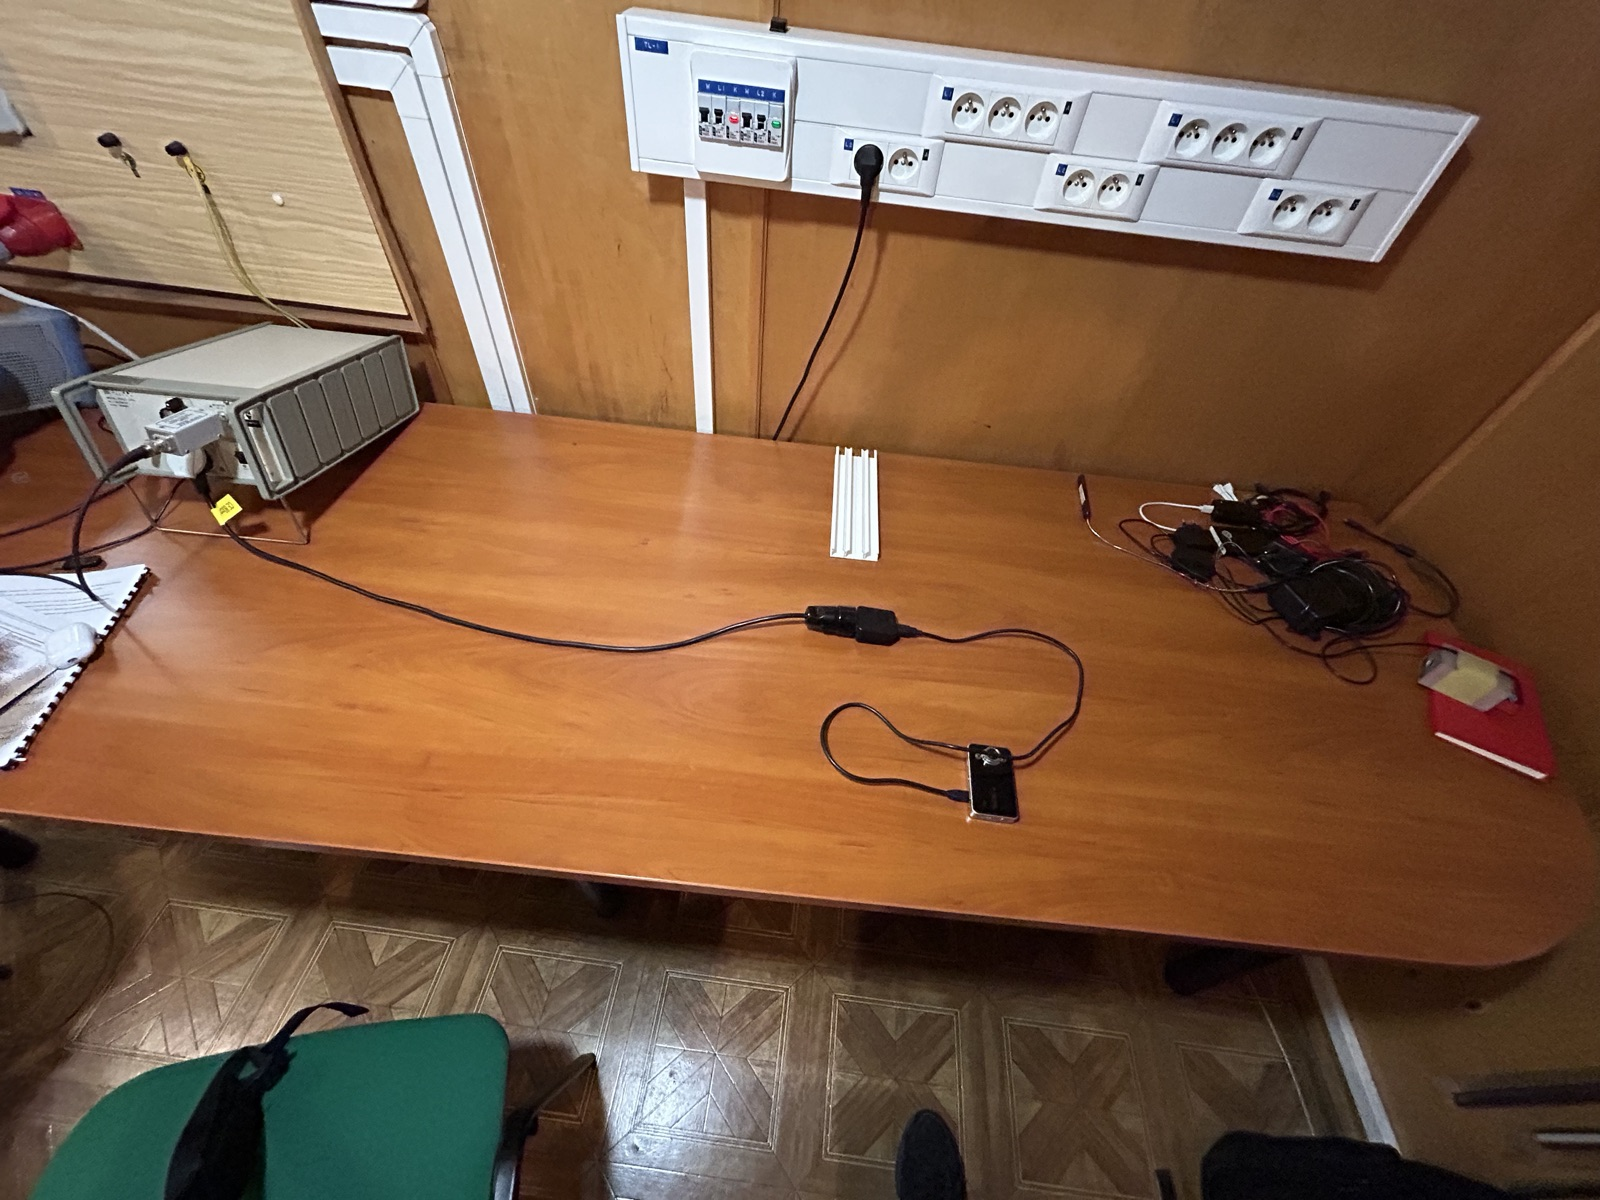
\includegraphics[width=\linewidth]{rys/stanowisko.jpg}\\
    {\small c) EUT podczas pomiaru 6}
  \end{minipage}
  \caption{Pomiar wstępny zasilacza USB-A bez obciążenia i~z~aparatem, linia L1.}
  \label{fig:ekr-aparat}
\end{figure}

\subsection{Zasilacz USB-A z~lampką LED}
\label{sec:lampka}

Po dołączeniu lampki poziom zaburzeń wzrósł względem tła o~ponad $40\ \mathrm{dB}$ (PK)
i~ok.~$33\ \mathrm{dB}$ (AV) (rys.~\ref{fig:ekr-lampka}). Ślad PK osiąga ok.~$80$--$84\ \dBuV$ w~paśmie
$0{,}15$--$0{,}5\ \mathrm{MHz}$ i~schodzi poniżej poziomu QP dopiero przy ok.~$3\ \mathrm{MHz}$ (linia N) i~$4\ \mathrm{MHz}$ (L1),
a~ślad AV przekracza swój poziom dopuszczalny do ok.~$1\ \mathrm{MHz}$.

Do $0{,}5\ \mathrm{MHz}$ widmo ma postać grzebienia regularnie rozmieszczonych prążków. Wyniki
pomiaru końcowego podano w~tabelach~\ref{tab:lampkaL1} i~\ref{tab:lampkaN}.

\begin{table}[H]
  \centering
  \small
  \begin{minipage}[t]{0.49\textwidth}\centering
    \captionof{table}{Wyniki pomiaru końcowego: zasilacz USB-A z~lampką LED, linia L1 (pomiar 8).}
    \label{tab:lampkaL1}
    \footnotesize\setlength{\tabcolsep}{1.9pt}
    \renewcommand{\arraystretch}{1.1}
    \begin{tabular}{rcrrrc}
      \toprule
      \naglKoncowy
      \midrule
      \tabinput{tabele/t_lampka_L1}
      \bottomrule
    \end{tabular}
  \end{minipage}\hfill
  \begin{minipage}[t]{0.49\textwidth}\centering
    \captionof{table}{Wyniki pomiaru końcowego: zasilacz USB-A z~lampką LED, linia N (pomiar 9).}
    \label{tab:lampkaN}
    \footnotesize\setlength{\tabcolsep}{1.9pt}
    \renewcommand{\arraystretch}{1.1}
    \begin{tabular}{rcrrrc}
      \toprule
      \naglKoncowy
      \midrule
      \tabinput{tabele/t_lampka_N}
      \bottomrule
    \end{tabular}
  \end{minipage}
\end{table}

\paragraph{Przykład obliczeń do tabeli~\ref{tab:lampkaL1}.} Dla detektora QP przy
$f = 426\ \mathrm{kHz}$, gdzie $U = 76{,}68\ \dBuV$:
\begin{align*}
  L_{QP} &= 66 - 10\cdot\frac{\log_{10}(0{,}426/0{,}15)}{\log_{10}(0{,}5/0{,}15)}
          = 66 - 10\cdot\frac{0{,}4533}{0{,}5229} = 66 - 8{,}67 = 57{,}33\ \dBuV,\\
  \Delta &= U - L_{QP} = 76{,}68\ \dBuV - 57{,}33\ \dBuV = +19{,}35\ \mathrm{dB}.
\end{align*}
Najwyższy zmierzony poziom, $80{,}22\ \dBuV$ (QP, $174\ \mathrm{kHz}$), odpowiada napięciu
$10{,}3\ \mathrm{mV}$, ok.~sześciokrotnie większemu od dopuszczalnego ($1{,}73\ \mathrm{mV}$).
Obliczone wartości $\Delta$ są zgodne z~raportem odbiornika.

W~paśmie $0{,}15$--$0{,}55\ \mathrm{MHz}$ przekroczenia wynoszą na linii L1
$9{,}7$--$19{,}4\ \mathrm{dB}$ (QP) i~$4{,}7$--$7{,}1\ \mathrm{dB}$ (AV), a~na linii N
$14{,}0$--$17{,}4\ \mathrm{dB}$ i~$2{,}9$--$5{,}3\ \mathrm{dB}$ (rys.~\ref{fig:wykres-lampka}).
Przekroczenia QP są kilkukrotnie większe od niepewności $U_{cispr} = 3{,}4\ \mathrm{dB}$, zatem
zasilacz USB-A z~lampką LED nie spełnia wymagań PN-EN~55032 dla klasy~B. Poziomy na linii L1 są
na ogół o~ok.~$2\ \mathrm{dB}$ wyższe niż na linii N.

\begin{figure}[H]
  \centering
  \begin{minipage}[t]{0.42\textwidth}\centering
    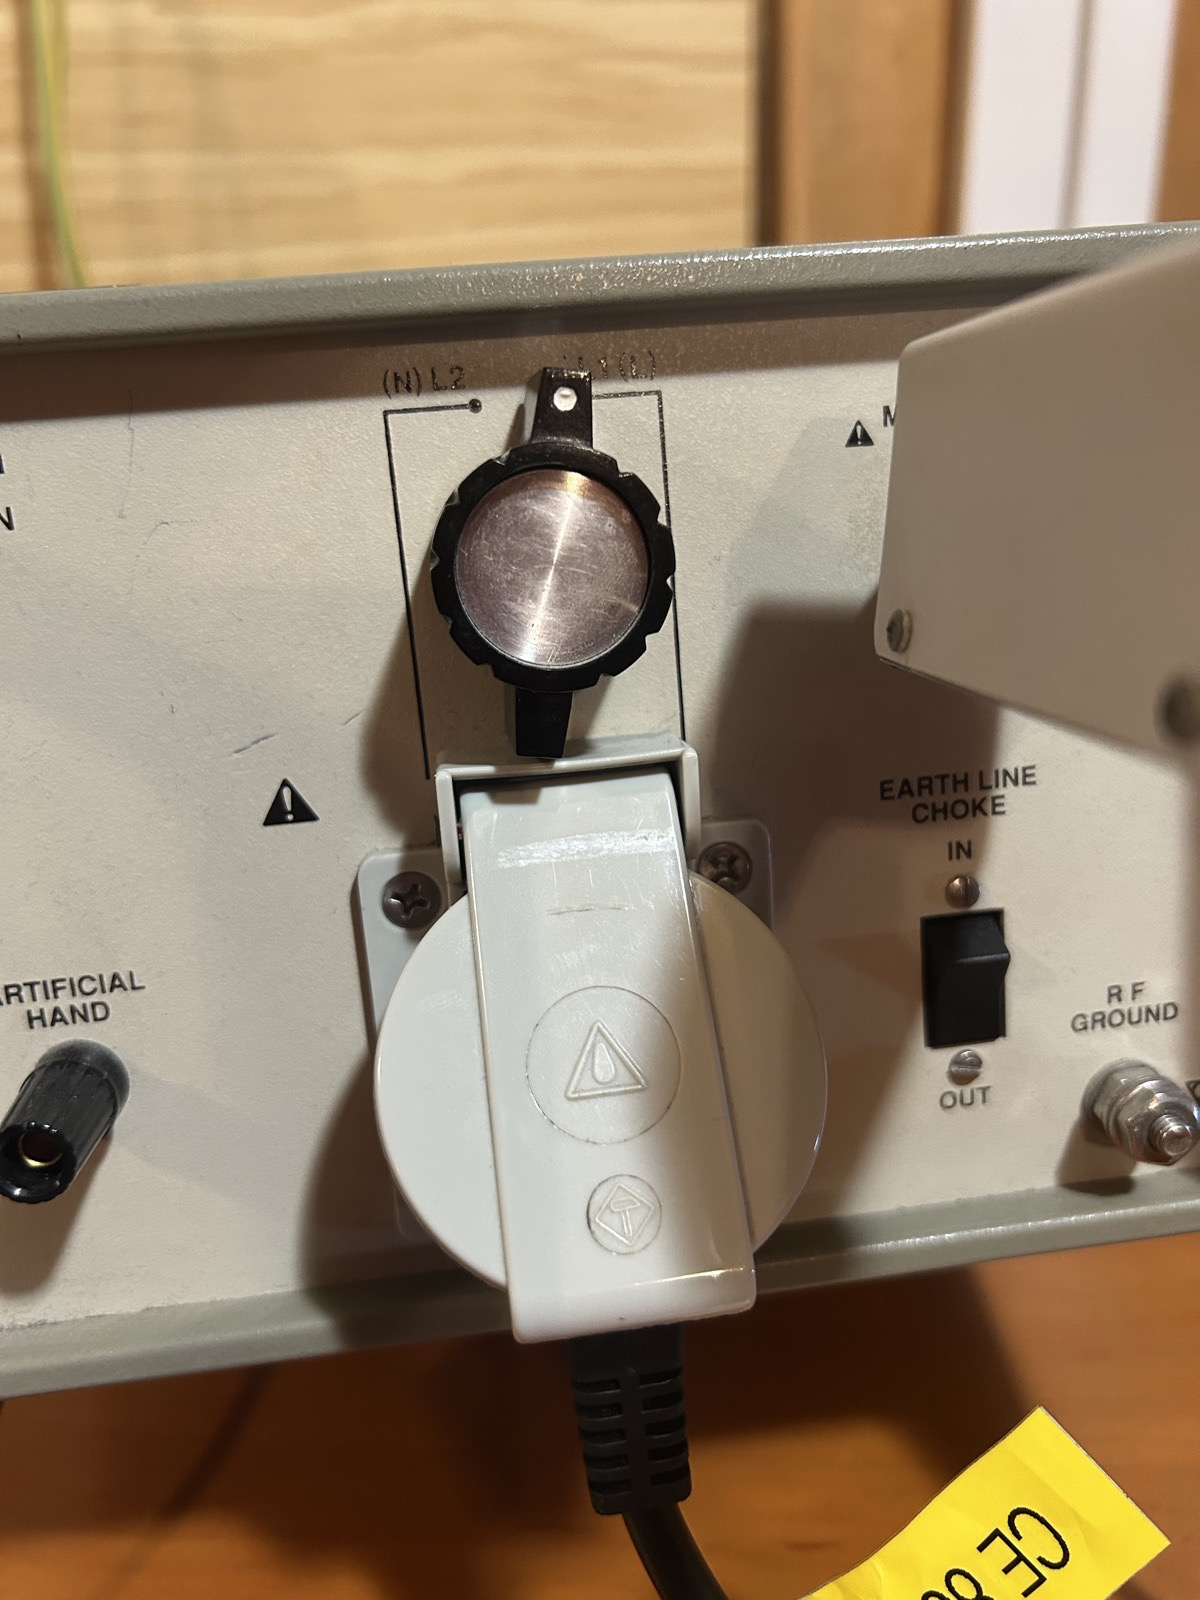
\includegraphics[height=6.8cm]{rys/przelacznik_L1.jpg}\\
    {\small a) położenie L1 (pomiar 8)}
  \end{minipage}\hspace{0.04\textwidth}
  \begin{minipage}[t]{0.42\textwidth}\centering
    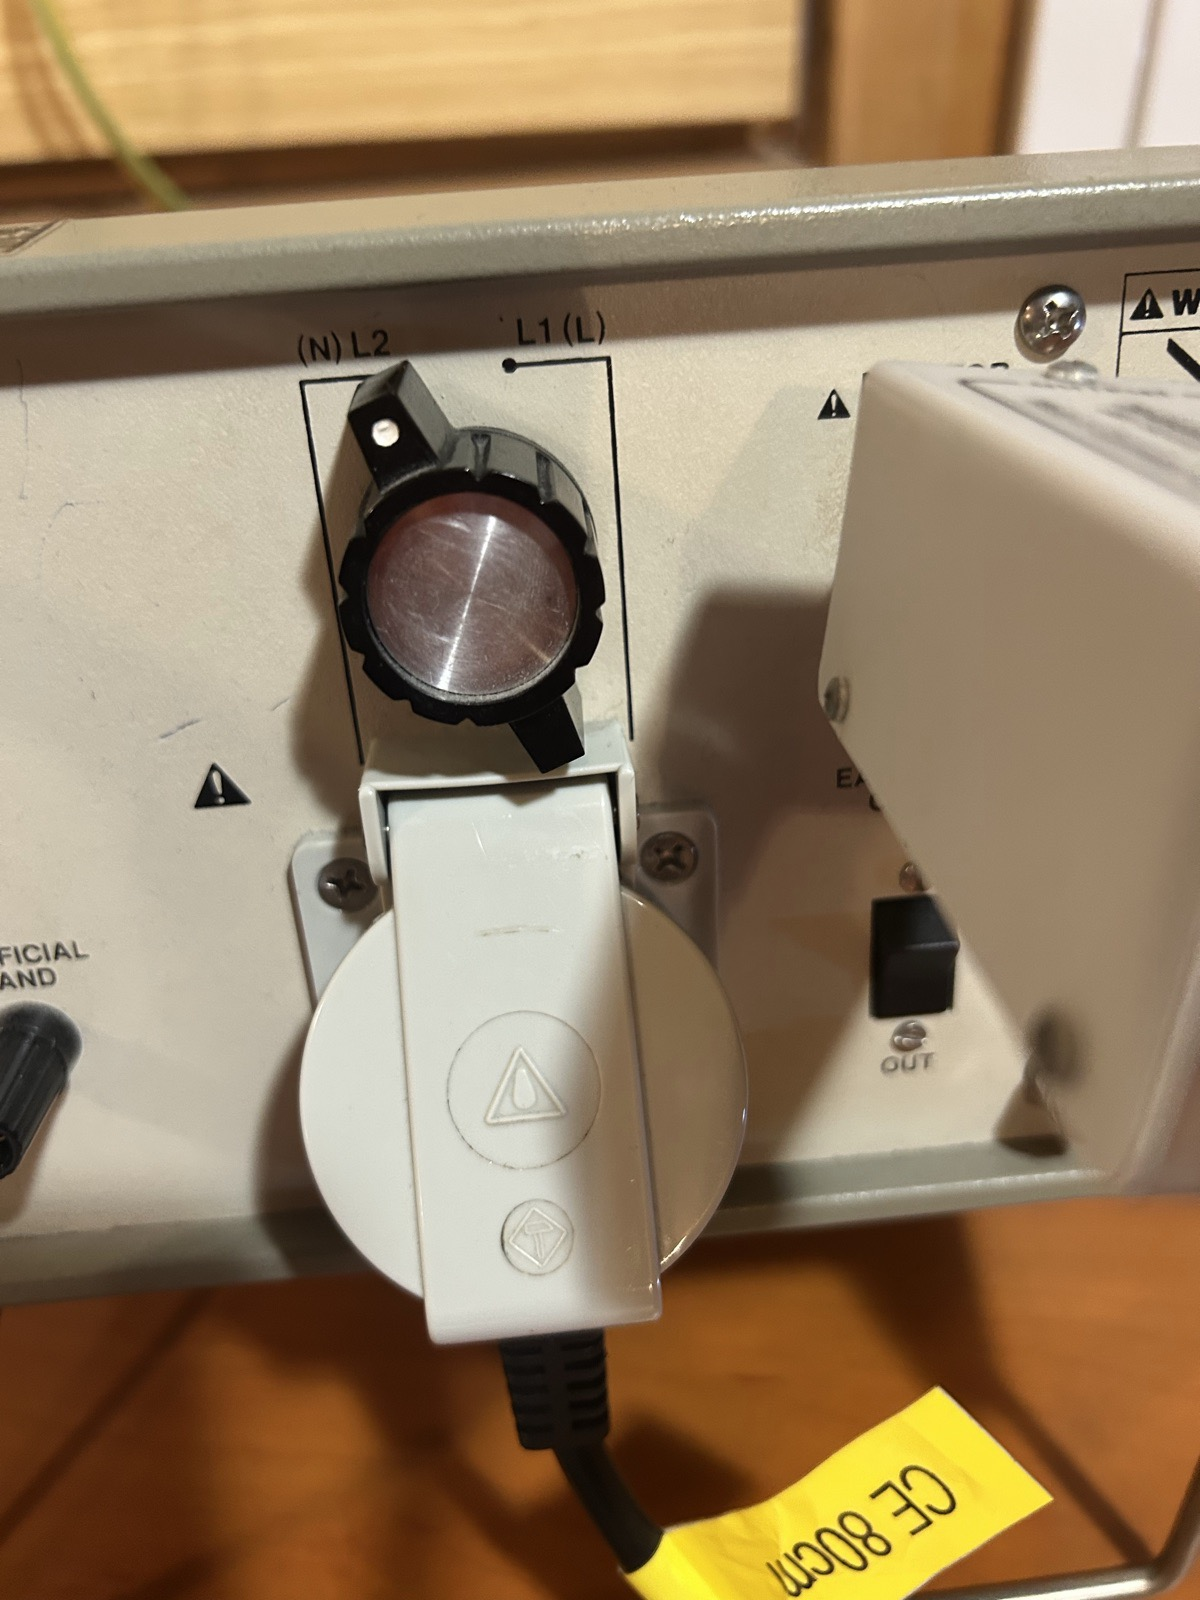
\includegraphics[height=6.8cm]{rys/przelacznik_N.jpg}\\
    {\small b) położenie N (L2) (pomiar 9)}
  \end{minipage}
  \caption{Przełącznik linii sieci sztucznej podczas pomiarów zasilacza USB-A z~lampką LED.}
  \label{fig:przelacznik}
\end{figure}

\begin{figure}[H]
  \centering
  \ekran{ekr_8_lampka_L1}{a) pomiar 8: linia L1}\hfill
  \ekran{ekr_9_lampka_N}{b) pomiar 9: linia N}
  \caption{Raport odbiornika dla zasilacza USB-A z~lampką LED na liniach L1 i~N. Znaki ,,+''
           i~,,$\times$'' oznaczają wyniki pomiaru końcowego detektorem QP i~AV.}
  \label{fig:ekr-lampka}
\end{figure}

\begin{figure}[H]
  \centering
  \begin{tikzpicture}
    \begin{axis}[xmode=log, wykres, height=7.4cm, ymin=30, ymax=90, legend columns=3, xmax=6,
                 xtick={0.15,0.2,0.3,0.5,1,2,3,5},
                 xticklabels={{0,15},{0,2},{0,3},{0,5},1,2,3,5}]
      \limity
      \addlegendimage{empty legend}\addlegendentry{}
      \addplot[only marks, mark=*, mark size=2.2pt, seriaA] table[x=f, y=U] {dane/lampka_L1_qp.dat};
      \addlegendentry{QP, linia L1}
      \addplot[only marks, mark=o, mark size=2.2pt, seriaA, thick] table[x=f, y=U] {dane/lampka_L1_av.dat};
      \addlegendentry{AV, linia L1}
      \addlegendimage{empty legend}\addlegendentry{}
      \addplot[only marks, mark=square*, mark size=2.0pt, seriaB] table[x=f, y=U] {dane/lampka_N_qp.dat};
      \addlegendentry{QP, linia N}
      \addplot[only marks, mark=square, mark size=2.0pt, seriaB, thick] table[x=f, y=U] {dane/lampka_N_av.dat};
      \addlegendentry{AV, linia N}
    \end{axis}
  \end{tikzpicture}
  \caption{Wyniki pomiaru końcowego zasilacza USB-A z~lampką LED na tle
           poziomów dopuszczalnych PN-EN~55032 klasy~B. Znaki pełne: detektor QP, puste:
           detektor AV.}
  \label{fig:wykres-lampka}
\end{figure}

\subsection{Zasilacz USB-A bez obciążenia (lampka niepodłączona)}
\label{sec:bez}

Bez lampki ślad PK w~paśmie $0{,}15$--$1\ \mathrm{MHz}$ miejscami przekracza poziom
QP, stąd wynik FAIL na ekranie odbiornika (rys.~\ref{fig:ekr-bez}). Wynik ten dotyczy jednak
wyłącznie pomiaru wstępnego.

W~pomiarze końcowym (tab.~\ref{tab:bezL1} i~\ref{tab:bezN}) wszystkie wartości QP znalazły się
poniżej poziomu dopuszczalnego, z~najmniejszym zapasem $5{,}4\ \mathrm{dB}$ na linii L1
($546\ \mathrm{kHz}$) i~$7{,}3\ \mathrm{dB}$ na linii N ($558\ \mathrm{kHz}$). Ślad AV
pozostawał blisko tła (najwyżej ok.~$5\ \mathrm{dB}$ powyżej). Zasilacz bez obciążenia spełnia zatem wymagania normy.

\begin{figure}[H]
  \centering
  \ekran{ekr_7_lampka_bez_L1}{a) pomiar 7: linia L1}\hfill
  \ekran{ekr_10_lampka_bez_N}{b) pomiar 10: linia N}
  \caption{Raport odbiornika dla zasilacza USB-A bez obciążenia (lampka niepodłączona).}
  \label{fig:ekr-bez}
\end{figure}

\begin{table}[H]
  \centering
  \small
  \begin{minipage}[t]{0.49\textwidth}\centering
    \captionof{table}{Wyniki pomiaru końcowego: zasilacz bez obciążenia, linia L1 (pomiar 7).}
    \label{tab:bezL1}
    \footnotesize\setlength{\tabcolsep}{3pt}
    \renewcommand{\arraystretch}{1.1}
    \begin{tabular}{rcrrrc}
      \toprule
      \naglKoncowy
      \midrule
      \tabinput{tabele/t_bez_L1}
      \bottomrule
    \end{tabular}
  \end{minipage}\hfill
  \begin{minipage}[t]{0.49\textwidth}\centering
    \captionof{table}{Wyniki pomiaru końcowego: zasilacz bez obciążenia, linia N (pomiar 10).}
    \label{tab:bezN}
    \footnotesize\setlength{\tabcolsep}{3pt}
    \renewcommand{\arraystretch}{1.1}
    \begin{tabular}{rcrrrc}
      \toprule
      \naglKoncowy
      \midrule
      \tabinput{tabele/t_bez_N}
      \bottomrule
    \end{tabular}
  \end{minipage}
\end{table}

Należy zauważyć, że w~pomiarach~7 i~10 zasilacz pracował bez przewodu i~obciążenia, tak jak
w~pomiarze~2, a~mimo to wystąpiły wyraźne prążki (QP do $54{,}6\ \dBuV$). W~pomiarach~2 i~5
przebieg pozostawał na poziomie tła. Nieregularne odstępy wyników na linii N
($16$--$84\ \mathrm{kHz}$) mogą świadczyć o~pracy przetwornicy bez obciążenia w~trybie
impulsowym (\emph{burst}), w~którym widmo zaburzeń jest niestabilne. Przyczyny różnicy nie
udało się jednoznacznie ustalić.

\subsection{Najmniejsze marginesy i~ocena zgodności}
\label{sec:zestawienie}

Dla każdego pomiaru wyznaczono częstotliwość, przy której margines do poziomu dopuszczalnego
jest najmniejszy, tzn.\ odstęp $\Delta$ jest największy (tab.~\ref{tab:zestawienie}). Wartości
z~pomiaru końcowego pochodzą z~plików \texttt{.DAT}. Pozostałe oszacowano ze zrzutów ekranu
pomiaru wstępnego, porównując ślad PK z~$L_{QP}$, a~ślad AV z~$L_{AV}$. Ponieważ
$U_{PK} \ge U_{QP}$, oszacowanie dla QP jest zachowawcze.

\begin{table}[H]
  \centering
  \small
  \caption{Najmniejsze marginesy do poziomów dopuszczalnych PN-EN~55032 klasy~B i~ocena
           zgodności. Wartości ze znakiem $\approx$ oszacowano ze zrzutów ekranu (dokładność
           ok.~$1\ \mathrm{dB}$), pozostałe pochodzą z~pomiaru końcowego.}
  \label{tab:zestawienie}
  \renewcommand{\arraystretch}{1.15}
  \setlength{\tabcolsep}{4pt}
  \begin{tabular}{|c|>{\raggedright\arraybackslash}p{5.6cm}|c|c|c|c|c|c|}
    \hline
    \textbf{Nr} & \textbf{Badane urządzenie, warunki pracy} & \textbf{Linia} &
      \multicolumn{2}{c|}{\textbf{QP} (wstępnie PK)} & \multicolumn{2}{c|}{\textbf{AV}} & \textbf{Ocena} \\
    \cline{4-7}
     & & & $f$ [MHz] & $\Delta$ [dB] & $f$ [MHz] & $\Delta$ [dB] & \\
    \hline
    1  & brak EUT (tło) & L1 & $3{,}1$ & $\approx -13$ & $3{,}1$ & $\approx -14$ & --- \\ \hline
    2  & zasilacz USB-A bez przewodu i~obciążenia & L1 & $3{,}1$ & $\approx -14$ & $3{,}2$ & $\approx -14$ & spełnia \\ \hline
    3  & ładowarka Apple bez obciążenia & L1 & $3{,}1$ & $\approx -14$ & $3{,}1$ & $\approx -14$ & spełnia \\ \hline
    4  & ładowarka Apple z~iPhone'em & L1 & $0{,}20$ & $\approx -6$ & $0{,}20$ & $\approx -12$ & spełnia \\ \hline
    5  & zasilacz USB-A bez obciążenia & L1 & $3{,}1$ & $\approx -13$ & $3{,}1$ & $\approx -14$ & spełnia \\ \hline
    6  & zasilacz USB-A z~aparatem & L1 & $3{,}3$ & $\approx -13$ & $3{,}1$ & $\approx -14$ & spełnia \\ \hline
    7  & zasilacz USB-A, lampka niepodłączona & L1 & $0{,}546$ & $-5{,}38$ & $0{,}55$ & $\approx -14$ & spełnia \\ \hline
    8  & zasilacz USB-A z~lampką LED & L1 & $0{,}426$ & $+19{,}35$ & $0{,}302$ & $+7{,}05$ & nie spełnia \\ \hline
    9  & zasilacz USB-A z~lampką LED & N  & $0{,}362$ & $+17{,}40$ & $0{,}242$ & $+5{,}33$ & nie spełnia \\ \hline
    10 & zasilacz USB-A, lampka niepodłączona & N  & $0{,}558$ & $-7{,}28$ & $3{,}1$ & $\approx -14$ & spełnia \\ \hline
  \end{tabular}
\end{table}

W~pomiarach~1--3, 5 i~6 najmniejszy margines wypada przy skoku tła ok.~$3\ \mathrm{MHz}$, wynika
więc z~tła, a~nie z~badanego urządzenia. Zasilacz USB-A z~lampką LED nie spełnia wymagań na
żadnej z~linii. W~pozostałych warunkach pracy wymagania są spełnione, a~najmniejszy zapas,
$5{,}38\ \mathrm{dB}$ (QP, pomiar~7), jest większy od niepewności $U_{cispr}$.

\subsection{Porównanie z~tłem oraz między warunkami pracy}
\label{sec:porownanie}

Ślady PK i~AV odczytano ze zrzutów ekranu w~funkcji częstotliwości i~wyznaczono ich największe
różnice (tab.~\ref{tab:porownanie}). Linie L1 i~N z~lampką porównano na podstawie wyników
końcowych, ponieważ prążki obu pomiarów leżą przy nieco innych częstotliwościach.

Przebiegi pomiarów~2, 3 i~5 różnią się od tła najwyżej o~kilka decybeli, z~wyjątkiem
wąskiego prążka przy ok.~$12\ \mathrm{MHz}$. W~pomiarze~6 wystąpiły ponadto wzniesienia do
ok.~$9\ \mathrm{dB}$ w~paśmie $18$--$28\ \mathrm{MHz}$. Prążek przy $12\ \mathrm{MHz}$ wystąpił tylko
w~kolejnych pomiarach~2--6, niezależnie od badanej ładowarki, a~nie było go w~tle ani
w~pomiarach~7 i~10, dlatego uznano go za zaburzenie pochodzące z~otoczenia.

Obciążenie zwiększa zaburzenia przede wszystkim w~paśmie $0{,}2$--$0{,}3\ \mathrm{MHz}$, tj.\ przy
niskich harmonicznych częstotliwości przełączania: o~ok.~$20\ \mathrm{dB}$ (PK) dla ładowarki
Apple i~o~$24$--$32\ \mathrm{dB}$ dla zasilacza z~lampką. Wyjątkiem jest aparat, po którego
podłączeniu wzrost (do $10\ \mathrm{dB}$ względem pomiaru~5) wystąpił tylko w~paśmie $18$--$28\ \mathrm{MHz}$.

Bez obciążenia poziom PK na linii L1 był wyższy niż na linii N o~maksymalnie $10\ \mathrm{dB}$
(ok.~$0{,}32\ \mathrm{MHz}$). Z~lampką wyniki końcowe na obu liniach różnią się zwykle
o~ok.~$2\ \mathrm{dB}$. Największą różnicę, $7{,}2\ \mathrm{dB}$ na korzyść linii N,
zaobserwowano przy 6.~harmonicznej ($342$/$362\ \mathrm{kHz}$).

\begin{table}[H]
  \centering
  \small
  \caption{Największe różnice poziomów zaburzeń: względem tła, między stanem z~obciążeniem
           i~bez obciążenia oraz między liniami L1 i~N. Wartości dodatnie oznaczają wyższy
           poziom w~pierwszym z~porównywanych pomiarów.}
  \label{tab:porownanie}
  \renewcommand{\arraystretch}{1.15}
  \begin{tabular}{|>{\raggedright\arraybackslash}p{7.2cm}|c|c|c|c|}
    \hline
    \textbf{Porównanie (nr pomiarów)} & \multicolumn{2}{c|}{\textbf{Ślad PK}} & \multicolumn{2}{c|}{\textbf{Ślad AV}} \\
    \cline{2-5}
     & $\Delta U_{max}$ [dB] & $f$ [MHz] & $\Delta U_{max}$ [dB] & $f$ [MHz] \\
    \hline
    \multicolumn{5}{|l|}{\textit{względem tła (pomiar 1)}} \\ \hline
    2 -- 1: zasilacz USB-A bez przewodu i~obciążenia & $\le 2$ & --- & $+3$ & $12$ \\ \hline
    3 -- 1: ładowarka Apple bez obciążenia & $\le 2$ & --- & $+5$ & $12$ \\ \hline
    4 -- 1: ładowarka Apple z~iPhone'em & $+19$ & $0{,}20$ & $+14$ & $0{,}20$ \\ \hline
    5 -- 1: zasilacz USB-A bez obciążenia & $+10$ & $12$ & $+12$ & $12$ \\ \hline
    6 -- 1: zasilacz USB-A z~aparatem & $+9$ & $19$ & $+7$ & $28$ \\ \hline
    7 -- 1: zasilacz USB-A, lampka niepodłączona, L1 & $+24$ & $0{,}56$ & $+5$ & $0{,}42$ \\ \hline
    8 -- 1: zasilacz USB-A z~lampką LED, L1 & $+46$ & $0{,}16$ & $+33$ & $0{,}27$ \\ \hline
    9 -- 1: zasilacz USB-A z~lampką LED, N & $+43$ & $0{,}26$ & $+33$ & $0{,}20$ \\ \hline
    10 -- 1: zasilacz USB-A, lampka niepodłączona, N & $+20$ & $0{,}37$ & $+3$ & $0{,}35$ \\ \hline
    \multicolumn{5}{|l|}{\textit{z~obciążeniem względem stanu bez obciążenia}} \\ \hline
    4 -- 3: ładowarka Apple, iPhone & $+20$ & $0{,}20$ & $+14$ & $0{,}22$ \\ \hline
    6 -- 5: zasilacz USB-A, aparat & $+10$ & $20$ & $+7$ & $28$ \\ \hline
    8 -- 7: zasilacz USB-A, lampka, L1 & $+24$ & $0{,}26$ & $+30$ & $0{,}27$ \\ \hline
    9 -- 10: zasilacz USB-A, lampka, N & $+31$ & $0{,}21$ & $+32$ & $0{,}20$ \\ \hline
    \multicolumn{5}{|l|}{\textit{linia L1 względem linii N}} \\ \hline
    7 -- 10: bez obciążenia & $+10$ & $0{,}32$ & $+3$ & $0{,}51$ \\ \hline
    8 -- 9: z~lampką (wyniki końcowe QP i~AV) & $-7{,}2$ & $0{,}34/0{,}36$ & $+2{,}2$ & $0{,}36/0{,}37$ \\ \hline
  \end{tabular}
\end{table}

\subsection{Źródło zaburzeń}
\label{sec:zrodlo}

Wyniki końcowe dla zasilacza z~lampką leżą w~pobliżu wielokrotności ok.~$60\ \mathrm{kHz}$
(np.\ $174$, $238$, $286$, $342$, $426\ \mathrm{kHz}$ na linii L1). Są to harmoniczne $n = 3$--$9$ częstotliwości
podstawowej, którą oszacowano metodą najmniejszych kwadratów z~22 wyników, przyjmując
$n_k = \mathrm{round}(f_k/60\ \mathrm{kHz})$:
\[
  f_p = \frac{\sum_k n_k f_k}{\sum_k n_k^2} = 59{,}96\ \mathrm{kHz} \approx 60\ \mathrm{kHz}.
\]
Wartość ta jest typowa dla przetwornic zaporowych (\emph{flyback}) w~małych zasilaczach.
Niewielki rozrzut ($57$--$62\ \mathrm{kHz}$) wynika z~kroku przemiatania ($4\ \mathrm{kHz}$) i~niestabilności
częstotliwości przełączania.

Prążki są harmonicznymi jednej częstotliwości, a~ich poziom zależy od obciążenia, dlatego
źródłem zaburzeń jest najprawdopodobniej przetwornica zasilacza, a~nie samo obciążenie. Z~lampką
grzebień harmonicznych przekracza poziom dopuszczalny, z~aparatem przebieg pozostaje bliski tła.

W~paśmie $0{,}2$--$5\ \mathrm{MHz}$ obwiednia śladu PK maleje z~częstotliwością.
Dopasowanie prostej do obwiedni na zrzutach pomiarów~8 i~9 daje nachylenie
ok.~$20$--$22\ \mathrm{dB/dek.}$, zgodne z~teoretycznym spadkiem $20\ \mathrm{dB/dek.}$ dla przebiegu
trapezowego i~typowe dla zaburzeń różnicowych. Poziomy na obu liniach różnią się tylko
o~ok.~$2\ \mathrm{dB}$, a~bez znajomości fazy nie można rozdzielić składowych DM i~CM
według zależności~\eqref{eq:dmcm}.

Ładowarka Apple, mimo zwykle większej mocy obciążenia, wytwarza przy $0{,}2\ \mathrm{MHz}$ zaburzenia
o~ok.~$23$--$25\ \mathrm{dB}$ niższe niż zasilacz USB-A z~lampką, co może wskazywać na brak skutecznego filtru wejściowego w~zasilaczu USB-A. Emisję można
ograniczyć kondensatorem~X i~dławikiem różnicowym (DM) oraz dławikiem skompensowanym
z~kondensatorami~Y (CM).

\FloatBarrier
\section{Wnioski}

\begin{itemize}
  \item Poziom tła był co najmniej ok.~$13\ \mathrm{dB}$ niższy od poziomów dopuszczalnych
        (najmniejszy margines przy $3{,}1\ \mathrm{MHz}$), co pozwoliło na ocenę zgodności.
        Przebiegi w~pomiarach~2, 3 i~5 nie różniły się od tła, poza prążkiem przy
        ok.~$12\ \mathrm{MHz}$ pochodzącym z~otoczenia.

  \item Zasilacz USB-A z~lampką LED nie spełnia wymagań PN-EN~55032 klasy~B. Na linii L1
        poziom dopuszczalny został przekroczony o~$19{,}35\ \mathrm{dB}$ dla detektora QP
        ($426\ \mathrm{kHz}$) i~o~$7{,}05\ \mathrm{dB}$ dla AV ($302\ \mathrm{kHz}$). Pozostałe
        konfiguracje spełniają wymagania normy, przy czym najmniejszy zapas,
        $5{,}38\ \mathrm{dB}$, uzyskano dla zasilacza bez obciążenia (QP, $546\ \mathrm{kHz}$).

  \item Wynik FAIL w~pomiarze wstępnym zasilacza bez obciążenia nie został potwierdzony
        pomiarem końcowym. Jest to zgodne z~teorią, ponieważ detektor PK wskazuje wartość nie
        mniejszą niż QP. Dla zasilacza z~lampką wartości QP były wyższe od AV o~ok.~$19$--$23\ \mathrm{dB}$, co
        świadczy o~impulsowym charakterze zaburzeń.

  \item Po dołączeniu obciążenia poziom zaburzeń w~paśmie $0{,}2$--$0{,}3\ \mathrm{MHz}$
        wzrósł o~$24$--$32\ \mathrm{dB}$ z~lampką i~o~ok.~$20\ \mathrm{dB}$ dla ładowarki
        Apple z~telefonem, co odpowiada oczekiwaniom dla zasilaczy impulsowych. Nie
        potwierdzono tego dla aparatu (wzrost jedynie powyżej $18\ \mathrm{MHz}$).
        Niewyjaśniona pozostała różnica między pomiarami~7 i~10 a~pomiarami~2 i~5,
        wykonanymi w~podobnych warunkach.

  \item Wyniki na liniach L1 i~N różniły się zwykle o~ok.~$2\ \mathrm{dB}$. Nachylenie obwiedni
        widma, ok.~$20$--$22\ \mathrm{dB/dek.}$, jest zgodne z~teoretycznym spadkiem
        $20\ \mathrm{dB/dek.}$ dla przebiegu trapezowego i~wskazuje na przewagę składowej
        różnicowej.

  \item Prążki leżą przy wielokrotnościach ok.~$60\ \mathrm{kHz}$, czyli są harmonicznymi częstotliwości
        przełączania. Za ich źródło uznano przetwornicę zasilacza USB-A, prawdopodobnie
        pozbawioną skutecznego filtru wejściowego.
\end{itemize}


% =====================================================================
{\small
\begin{thebibliography}{9}
\setlength{\itemsep}{1pt}
\bibitem{instr} M.~E.~Szafrańska, M.~Macko, D.~Kaliszuk, M.~Michalak, \emph{Instrukcja do
  ćwiczenia nr~2: Pomiary przewodzonych zaburzeń elektromagnetycznych za pomocą sieci
  sztucznej}, Laboratorium Kompatybilności Elektromagnetycznej i~Bezpieczeństwa
  Elektromagnetycznego, Katedra Telekomunikacji i~Teleinformatyki, Politechnika Wrocławska,
  Wrocław 2024.
\bibitem{esl} M.~Macko, D.~Kaliszuk, A.~J.~Pomianek, \emph{Uproszczona instrukcja obsługi
  odbiornika pomiarowego R\&S ESL3 EMI Test Receiver}, Laboratorium Kompatybilności
  Elektromagnetycznej, Politechnika Wrocławska, Wrocław 2012, rev.~2 2024.
\bibitem{pn16-2-1} PN-EN~55016-2-1, \emph{Wymagania dotyczące aparatury pomiarowej i~metod
  pomiaru zaburzeń radioelektrycznych oraz odporności na zaburzenia -- Część 2-1: Metody
  pomiaru zaburzeń i~badania odporności -- Pomiary zaburzeń przewodzonych}.
\bibitem{pn16-4-2} PN-EN~55016-4-2, \emph{Wymagania dotyczące aparatury pomiarowej i~metod
  pomiaru zaburzeń radioelektrycznych oraz odporności na zaburzenia -- Część 4-2:
  Niepewności, statystyka i~modelowanie poziomów dopuszczalnych -- Niepewność aparatury
  pomiarowej}.
\bibitem{pn55032} PN-EN~55032, \emph{Kompatybilność elektromagnetyczna urządzeń
  multimedialnych -- Wymagania dotyczące emisji}.
\bibitem{williams} T.~Williams, \emph{Conducted Interference}, Elmac Services (materiały
  udostępnione na ePortalu).
\bibitem{smps} T.~Williams, \emph{Emissions measurements on switch-mode power supplies},
  Elmac Services (materiały udostępnione na ePortalu).
\end{thebibliography}
}

\end{document}
